\documentclass[12pt,fleqn]{article}\usepackage{../../common}
\begin{document}
Materyel Mekaniği - 6

Direk Direngenlik Metotu (Direct Stiffness Method)

Direngenlik metotunu anlamak için direngenlik matrisi kavramını işlemek
gerekir. Bu konuya biraz [2]'de değindik. Bir öğe grubunun, sistemin direngenlik
matrisi düğümsel yer değişimler $d$ ile düğümsel kuvvetler $F$'yi ilintilendiren
bir $K$ matrisidir, öyle ki [1, sf. 34]

$$
F = K d
$$

eşitliği geçerlidir. Alttaki gibi bir sistem olsun,

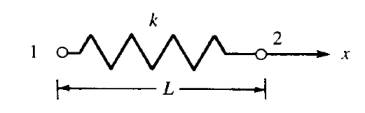
\includegraphics[width=15em]{phy_020_strs_06_03.jpg}

Sistemde bir yay görülüyor, bu yay üzerinde iki tane düğüm noktası seçtik,
onları takip edeceğiz, düğüm 1 ve 2. Düğümlerdeki yer değişimler $u_1,u_2$
olsun, yaydaki toplam değişimo $\delta = u_1 - u_2$. Uygulanan kuvvet $T$
ise bir sabit $k$ üzerinden $T = k \delta$ eşitliği ortaya atılabilir.

Direngenlik matrisine gelirsek, sistemdeki tum yer degisimleri soyle gosterebiliriz,

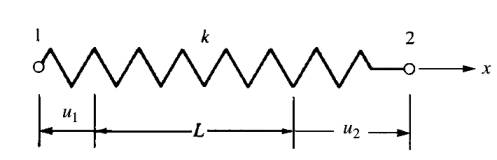
\includegraphics[width=15em]{phy_020_strs_06_04.jpg}

Sağ uçta yay $T$ kuvveti ile çekiliyorsa, bu durum sol uçta $-T$ tepkisel
kuvvete sebep olur. Ayrıca $u_1$'in sol yönü işaret ettiğine dikkat, çünkü yer
değişimin yönü pozitif yönün tersinde, yaydaki takip edilen nokta başlangıç
anının sol tarafında kalıyor, bu sebeple yön eksi.

$$
f_{1x} = -T, \quad f_{2x} = T
$$

Hepsini bir araya koyarsak

$$
T = -f_{1x} = k (u_2 - u_1)
$$

$$
T = f_{2x} = k (u_2 - u_1)
$$

Yani

$$
f_{1x} = k(u_1 - u_2)
$$

$$
f_{2x} = k(u_2 - u_1)
$$

Matris formunu kullanarak,

$$
\left[\begin{array}{ccc}
f_{1x} \\ f_{2x}
\end{array}\right] = 
\left[\begin{array}{ccc}
k & -k \\ -k & k
\end{array}\right]
\left[\begin{array}{ccc}
u_1 \\ u_2
\end{array}\right]
$$

İfadenin ortasındaki 2 x 2 matrisi direngenlik matrisidir.

Üstdüşüm (Superposition)

Eğer iki tane yay sistemini birbiriyle bağlı olarak işlemek istersek [1, sf. 38],
üstdüşüm tekniği kullanılabilir. Üstdüşüm basit bir matris toplamı ile
yapılabiliyor. Alttaki örneğe bakalım,

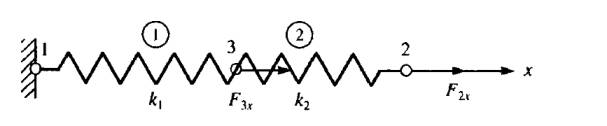
\includegraphics[width=20em]{phy_020_strs_06_02.jpg}

İki yay var, birbirlerine bağlılar, iki yayın sabitleri $k_1$, $k_2$
olsun. Her iki yayın direngenlik matrisi ayrı ayrı (tekabül eden yer değişim
değişkenleri matris kolon etiketi olarak gösteriliyor),

$$
k^{(1)} =
\begin{array}{cc} & \begin{array}{cc} u_1 & u_3 \end{array} \\ &
\left[
\begin{array}{cc}
k_1 & -k_1 \\ -k_1 & k_1
\end{array}
\right]
\end{array} 
\qquad
k^{(2)} =
\begin{array}{cc} & \begin{array}{cc} u_3 & u_2 \end{array} \\ &
\left[
\begin{array}{cc}
k_2 & -k_2 \\ -k_2 & k_2
\end{array}
\right]
\end{array}
$$

İki yay sistemini tek sistem haline getirmek aslında basit bir matris
toplamından ibaret fakat bu matrisin kolonları aynı değişkenlere tekabül ediyor
olmalı. O zaman her iki 2 x 2 matrisi genişletip 3 x 3 matrisi haline
getirirsek, değişken etiketlerini eşitlersek bu yeni iki matrisi
toplayabiliriz.

$$
k^{(1)} =
\begin{array}{cc} & \begin{array}{ccc} u_1 & u_2 & u_3 \end{array} \\ &
\left[
\begin{array}{ccc}
k_1 & 0 & -k_1 \\
0 & 0 & 0 \\
-k_1 & 0 & k_1
\end{array}
\right]
\end{array} \qquad
k^{(2)} =
\begin{array}{cc} & \begin{array}{ccc} u_1 & u_2 & u_3 \end{array} \\ &
\left[
\begin{array}{ccc}
0 & 0 & 0 \\
0 & k_2 & -k_2 \\
0 & -k_2 & k_2
\end{array}
\right]
\end{array} \qquad
$$

Dikkat edilirse mesela ilk matrisin $u_2$ kolonu tamamen sıfır çünkü 2 x 2
halindeki $k^{(1)}$ matrisinde bu değişken yoktu. Yeni genişletilmiş matrise
geçerken olmayan değişkenin kolonunu sıfırlarsak aslında aynı matrisi elde etmiş
oluruz.

Artık iki matrisi toplayabiliriz,

$$
\left[\begin{array}{ccc}
k_1 & 0 & -k_1 \\
0 & k_2 & -k_2 \\
-k_1 & -k_2 & k_1+k_2
\end{array}\right]
\left[\begin{array}{c}
u_1 \\ u_2 \\ u_3
\end{array}\right] =
\left[\begin{array}{c}
F_{1x} \\ F_{2x} \\ F_{3x}
\end{array}\right]
$$

Sınır Şartları (Boundary Conditions)

Resimde gösterilen örnekte sol tarafın duvara sabitlendiğini görüyoruz.
Sabitlenme demek notasyonumuz itibariyle $u_1 = 0$ demektir. Bu bir
sınır şartıdır, onu bir şekilde sistemimize dahil etmemiz gerekir.
Değeri üstteki sistemde yerine koyarsak,

$$
\left[\begin{array}{ccc}
k_1 & 0 & -k_1 \\
0 & k_2 & -k_2 \\
-k_1 & -k_2 & k_1+k_2
\end{array}\right]
\left[\begin{array}{c}
0 \\ u_2 \\ u_3
\end{array}\right] =
\left[\begin{array}{c}
F_{1x} \\ F_{2x} \\ F_{3x}
\end{array}\right]
$$

Matris sistemini cebirsel olarak tekrar açarsak,

$$
k_1(0) + (0) u_2 - k_1 u_3 = F_{1x}
$$

$$
0(0) + k_2 u_2 - k_2 u_3 = F_{2x}
$$

$$
-k_1 (0) - k_2 u_2 + (k_1+k_2) u_3 = F_{3x}
$$

elde edilir. Bu sistemde sadece ikinci ve üçüncü denklemi matris olarak
yazabiliriz,

$$
\left[\begin{array}{cc}
k_2 & -k_2 \\ -k_2 & k_1 + k_2 
\end{array}\right]
\left[\begin{array}{c}
u_1 \\ u_2
\end{array}\right] =
\left[\begin{array}{c}
F_{2x} \\ F_{3x}
\end{array}\right]
$$

Bu son matrisi elde etmek için bir anlamda önceki matrisin birinci satırı ve
kolonunu dışarı attık, kenara ayırdık, ve kalanlarla yeni bir sistem yarattık.
Fakat dikkat bu $F_{1x}$ sıfır demek değildir, onun hala bir ifadesi var,
$F_{1x} = -k_1 u_3$, ve bu eşitliği bir kez sistemin geri kalanının çözdükten
sonra dönüp ayrıca bulmamız gerekiyor.

Devam edelim, yeni sistemi çözersek,

$$
\left[\begin{array}{ccc}
u_2 \\ u_3
\end{array}\right] =
\left[\begin{array}{cc}
k_2 & -k_2 \\ -k_2 & k_1 + k_2 
\end{array}\right]^{-1}
\left[\begin{array}{c}
F_{2x} \\ F_{3x}
\end{array}\right]
$$

$$
= \left[\begin{array}{cc}
\dfrac{1}{k_2} + \dfrac{1}{k_1} & \dfrac{1}{k_1} \\
\dfrac{1}{k_1} & \dfrac{1}{k_1} 
\end{array}\right]
\left[\begin{array}{c}
F_{2x} \\ F_{3x}
\end{array}\right]
$$

$u_2,u_3$ bir kez elde edildikten sonra $F_{1x} = -k_1 u_3$ formulu
ile $F_{1x}$ elde edilebilir.


[devam edecek]



Kaynaklar

[1] Logan, {\em A First Course in the Finite Element Method}

[2] Bayramlı, {\em Hesapsal Bilim, Ders 1-8}

\end{document}
